\chapter{Spectral Analysis of Directed Acyclic Graphs}
\label{ch:09-spectral-analysis-dags}

\lecturemeta{Isidora Stankovi\'{c}}{Faculty of Electrical Engineering, University of Montenegro}

One obstruction, one construction, one proof that the construction costs nothing. Graph signal processing supplies a Fourier transform by
diagonalising the adjacency matrix, and on a directed acyclic graph that machinery fails
completely, because a DAG's adjacency matrix is nilpotent and therefore has every eigenvalue
equal to zero. Stankovi\'{c}'s answer is to add a return edge to close the graph into a cycle,
which restores a spectrum, and then to insert enough zero-valued vertices along that return path
that the feedback it introduces cannot reach the original vertices within the filter's horizon.
The spectrum comes back and the filter output on the original graph is unchanged.

\section*{Key ideas}

\paragraph{Why anyone should care about DAG spectra.} DAGs are everywhere in machine learning:
computation graphs, causal and Bayesian networks, and autoregressive models, where causal
attention is precisely a DAG. The graph Fourier transform is the basis for spectral GNNs and for
graph filtering, so if it degenerates on DAGs then an entire toolkit is unavailable on a class of
graphs we use constantly.

\paragraph{The setup, in one paragraph.} For a directed graph $G = (V,E)$ with $|V| = N$ and
adjacency matrix $\Adj$, a graph signal is $\gsig = [x(1), \dots, x(N)]\T$. The shift operator is
the adjacency matrix itself, and a linear graph system is a polynomial in it,
\[
  H = \sum_{s=0}^{S} h_s \Adj^{s}, \qquad y = H\gsig = \sum_{s=0}^{S} h_s \Adj^{s}\gsig,
\]
\noindent where $\Adj^{s}$ describes propagation along directed paths of length $s$. This is
graph convolution: $\Adj\gsig$ is one message-passing hop and the $h_s$ are exactly the
coefficients a spectral GNN learns. If $\Adj = \Vmat \Lam \Vmat\inv$ is diagonalisable, the GFT is
$X = \Vmat\inv \gsig$ and the system acts multiplicatively in the spectral domain,
$H(\Lam) = \sum_s h_s \Lam^{s}$.

\paragraph{The obstruction is structural, not numerical.} Topologically order a DAG's vertices
and its adjacency matrix becomes strictly upper triangular, which the lecture notes has the same
shape as a causal attention mask. A strictly upper triangular matrix is nilpotent,
$\Adj^{K} = \vect{0}$ for large enough $K$, so every eigenvalue is zero and $\Lam = \vect{0}$.
The consequence is not a loss of precision but a total collapse:
\[
  H(\Lam) = \sum_{s=0}^{S} h_s \Lam^{s} = h_0 \id,
\]
\noindent so every graph mode has the identical gain $h_0$, spectral components become
indistinguishable, frequency ordering disappears, and the adjacency-based GFT loses all
interpretability. What survives is vertex-domain propagation: $\Adj^{s}\gsig$ is still perfectly
meaningful. The spectrum, not the graph, is what breaks.

\begin{figure}[htbp]
\centering
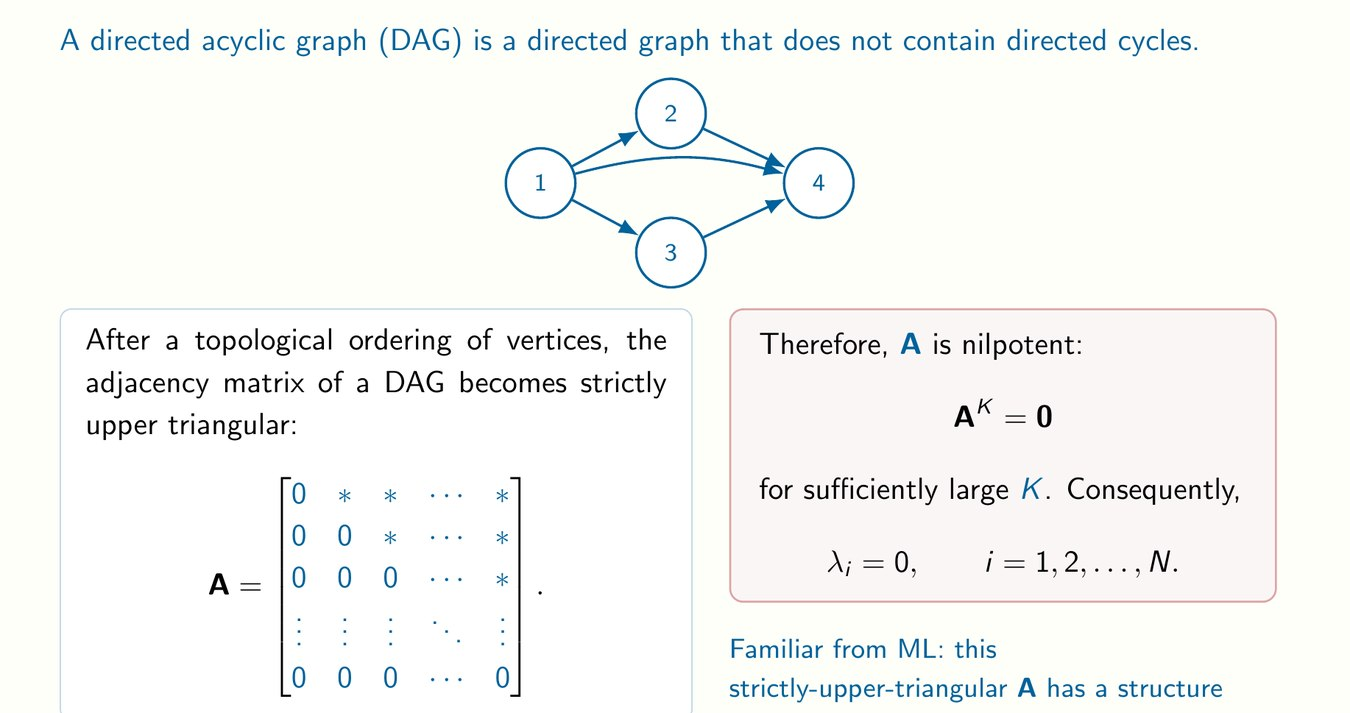
\includegraphics[width=0.86\textwidth]{figures/spectral-analysis-dags-1.jpg}
\caption{Where the obstruction comes from, from the Spectral Analysis of DAGs lecture. Topologically
ordering a DAG's vertices makes the adjacency matrix strictly upper triangular, which forces
$\Adj^{K} = \vect{0}$ and hence $\lambda_i = 0$ for every $i$. The lecture's own aside, bottom right: this is the same
matrix structure as a causal attention mask, so every decoder-only transformer has the same
degenerate spectrum.}
\label{fig:spectral-analysis-dags-1}
\end{figure}

\paragraph{Zero-padding, and the analogy that motivates it.} The construction is borrowed from
classical DFT practice (Figure~\ref{fig:spectral-analysis-dags-2}). A finite signal has no
spectrum until it is extended periodically, which introduces circular wrap-around; zero-padding is
how signal processing prevents that wrap-around from contaminating the interval of interest. The
graph version runs in three steps. A directed path has no spectrum because propagation does not
wrap around. Add a return edge from sink to source and the graph becomes a cycle, whose adjacency
eigenvalues are $\lambda_k = e^{j 2\pi (k-1)/N}$ with complex-exponential eigenvectors, so graph
spectral analysis on the cycle coincides exactly with the classical DFT. But the return edge is
feedback. So insert $M \ge S$ zero-valued vertices along it, which delay that feedback past the
horizon of any filter of order $S$.

\begin{figure}[htbp]
\centering
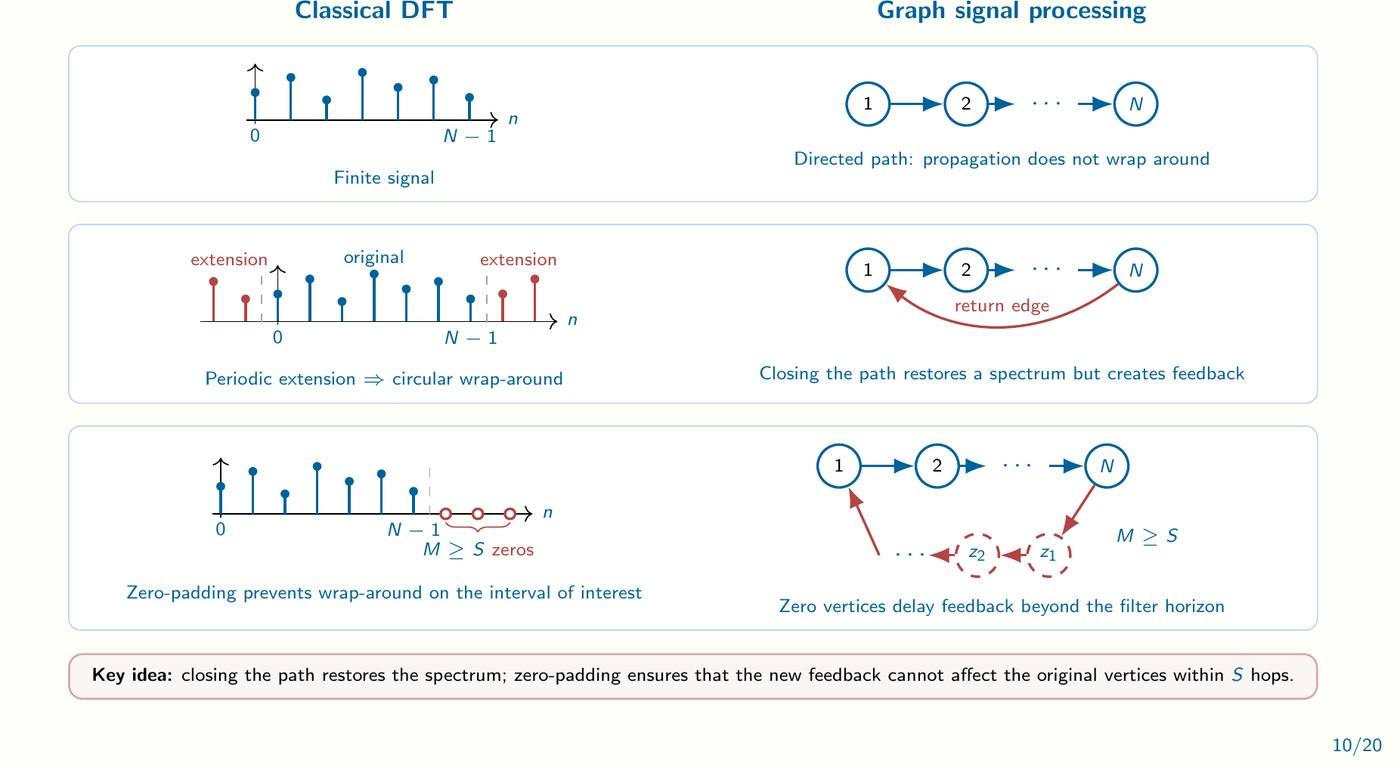
\includegraphics[width=0.92\textwidth]{figures/spectral-analysis-dags-2.jpg}
\caption{The construction and the analogy it comes from, from the Spectral Analysis of DAGs
lecture. Left column, classical DFT: a finite signal has no spectrum, periodic extension supplies
one at the cost of circular wrap-around, and zero-padding pushes that wrap-around outside the
interval of interest. Right column, the graph version step for step: a directed path does not wrap
around, a sink-to-source return edge closes it and restores a spectrum but introduces feedback, and
$M \ge S$ zero vertices $z_1, z_2, \dots$ along the return path delay that feedback beyond the
horizon of any order-$S$ filter.}
\label{fig:spectral-analysis-dags-2}
\end{figure}

\paragraph{The guarantee, and why the cycle is not cheating.} The augmented graph is cyclic on
purpose; the original object is still a DAG and the larger graph is a spectral embedding used only
for the transform. The formal statement is that for $0 \le s \le S$,
\[
  \bigl(\azp^{s} \gsig_{\mathrm{ZP}}\bigr)_{1:N} = \Adj^{s}\gsig,
  \qquad \gsig_{\mathrm{ZP}} = \begin{bmatrix} \gsig \\ \vect{0}\end{bmatrix},
\]
\noindent so filter outputs on the original vertices satisfy
$y_{\mathrm{ZP}}(1{:}N) = y$ exactly. After padding, $\azp$ has determinant $\pm 1$ and so is
invertible, meaning no eigenvalue is zero; the eigenvalue angle $\omega_k = \arg\{\lambda_k\}$
becomes the graph frequency, with slow modes at small angles and fast modes at large ones, and a
Fourier-like interpretation is restored. Diagonalisability additionally needs distinct
eigenvalues, which the talk checks exhaustively rather than assuming: over all connected DAGs on
7 vertices, a bare sink-to-source edge gives 98.4\% diagonalisable and one padding vertex gives
99.97\%; on 8 vertices, 99.0\% and, with two padding vertices, 99.91\%. The residual cases resolve
by giving the added edge weight $0.5$.

\begin{figure}[htbp]
\centering
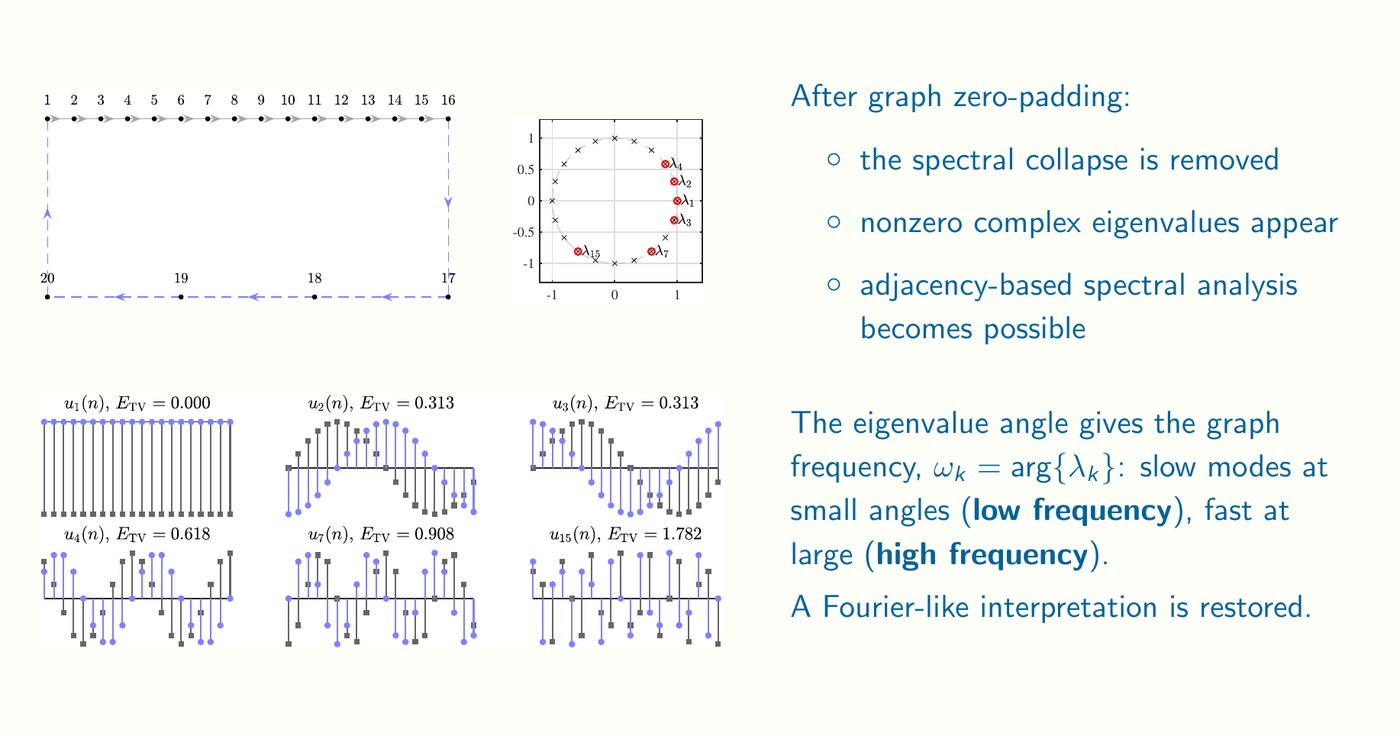
\includegraphics[width=0.92\textwidth]{figures/spectral-analysis-dags-3.jpg}
\caption{What is recovered, from the Spectral Analysis of DAGs lecture. Top left, a zero-padded
graph on 16 original vertices with the padding path closing it. Top middle, the resulting
eigenvalues, now nonzero complex numbers spread around the unit circle rather than all collapsed at
the origin. Bottom left, the corresponding eigenvectors ordered by total variation $E_{\mathrm{TV}}$,
from a constant mode at $0.000$ to a rapidly oscillating one at $1.782$, which is exactly the
low-to-high frequency ordering a Fourier basis is supposed to provide.}
\label{fig:spectral-analysis-dags-3}
\end{figure}

\paragraph{General DAGs, and the cost.} A single return edge suffices only when one directed
Hamiltonian path visits every vertex. A general DAG has several sources and sinks and no such
path, so the pipeline is two-stage: connect the DAG so a Hamiltonian path exists, then pad every
added edge. The overhead is linear, $N_{\mathrm{ZP}} = N + (K+1)M$ vertices for $K$ connecting
edges with $M$ padding vertices each. The worked application is denoising: a graph filter designed
in the restored spectral domain preserves the smoothest spectral components while attenuating
noise-dominated ones, taking a synthetic example from $\snr_{\mathrm{in}} = -6.99$ dB to
$\snr_{\mathrm{out}} = 6.21$ dB (Figure~\ref{fig:spectral-analysis-dags-4}).

\begin{figure}[htbp]
\centering
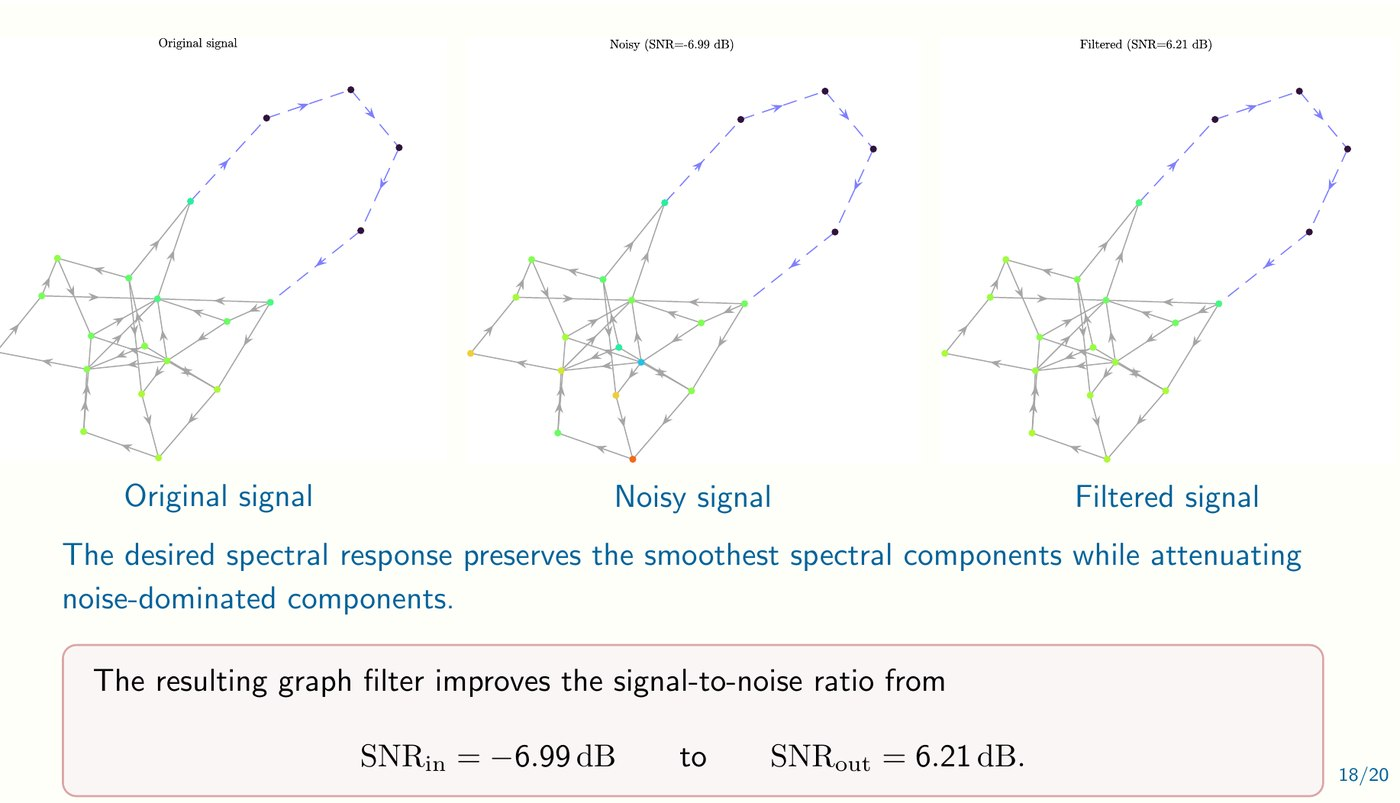
\includegraphics[width=0.92\textwidth]{figures/spectral-analysis-dags-4.jpg}
\caption{The payoff, from the Spectral Analysis of DAGs lecture. The same DAG carrying a smooth
signal, that signal with noise added, and the result of applying a low-pass graph filter designed in
the restored spectral domain. Vertex colour is signal value. The filter is only expressible because
zero-padding gave the DAG a spectrum to design in, and it recovers roughly 13 dB.}
\label{fig:spectral-analysis-dags-4}
\end{figure}

\section*{Notation}

$\Adj$ is the adjacency matrix, $\azp$ its zero-padded counterpart, $\Vmat$ and $\Lam$ the
eigenvector and eigenvalue matrices, $\gsig$ a graph signal, $h_s$ filter coefficients, $S$ the
filter order and $M$ the number of padding vertices. Note the collision with
Chapter~\ref{ch:04-intro-reinforcement-learning}, where $S$ is the state space; here $S$ is a
filter order, following each speaker's own usage.

\section*{Why it matters}

The lecture's own hook, that a strictly upper triangular adjacency matrix looks like a causal
attention mask, is the connection to chase. It means every decoder-only transformer is a DAG
whose spectral analysis is currently unavailable, and this construction is a candidate route to
it. That places the talk directly between Dieleman's spectral view of diffusion
(Chapter~\ref{ch:03-diffusion-models}), which treats the spectrum as the object being generated,
and Veli\v{c}kovi\'{c}'s geometric deep learning (Chapter~\ref{ch:11-geometric-deep-learning}),
where the graph Fourier transform underwrites spectral GNNs. It is also a good model of a small,
complete contribution: an obstruction, a fix, a proof that the fix is free, and an exhaustive
check of the one assumption that could fail.

\begin{aside}
The construction's soft spot is not the spectrum but the requirement of distinct eigenvalues. Instead
of assuming genericity, the talk enumerates all $2^{21}$ connected DAGs on eight vertices and reports
the failure rate. A complete enumeration on small instances costs an afternoon.
\end{aside}
